\section{Second Harmonic Generation Optical Rotation Solely Attributable to Chirality in Plasmonic Metasurfaces}\label{sec:results:OAinPlanarNanohelices}
This section has largely been copied verbatum from the manuscript \textit{``Second Harmonic Generation Optical Rotation Solely Attributable to Chirality in Plasmonic Metasurfaces''}, Joel~T.~Collins et. al. \cite{Collins2018b}. 
V. K. Valev designed the nonlinear experimental setup. A.G.Mark fabricated the samples. SHG data were collected by myself, and D. C. Hooper. Linear optical data were collected by myself and C. Kuppe. I analysed both the SHG and linear data. I produced the first draft of the manuscript, and all authors subsiquently contributed.
\\

Chiral plasmonic nanostructures, those lacking mirror symmetry, can be designed to manipulate the polarization of incident light resulting in chiroptical (chiral optical) effects such as circular dichroism (CD) and optical rotation (OR). Due to high symmetry sensitivity, corresponding effects in second harmonic generation (SHG-CD and SHG-OR) are typically much stronger in comparison. These nonlinear effects have long been used for chiral molecular analysis and characterization, however both linear and nonlinear optical rotation can occur even in achiral structures, if the structure is birefringent due to anisotropy. Crucially, chiroptical effects resulting from anisotropy typically exhibit a strong dependence on structural orientation. Here we report large second-harmonic generation optical rotation of $\pm\SI{45}{\degree}$, due to intrinsic chirality in a highly anisotropic helical metamaterial. The SHG intensity is found to strongly relate to the structural anisotropy, however the angle of SHG-OR is invariant under sample rotation. We show that by tuning the geometry of anisotropic nanostructures, the interaction between anisotropy, chirality, and experiment geometry can allow even greater control over the chiroptical properties of plasmonic metamaterials.

\subsection{Introduction}\label{sec:results:OAinPlanarNanohelices:introduction}
Modern nanofabrication techniques have allowed the development of optical “metamaterials”, whose properties are determined not only by the choice of materials, but also by their geometry. The strong dependence on geometry enables the design of metamaterials exhibiting tailored optical properties.\cite{Pendry2004a, Alu2007, Kauranen2012, Meinzer2014, Moitra2015, Cong2015, Prudencio2016}. 
Optical metamaterials, consisting of sub-wavelength metallic nanostructures, can greatly benefit from surface plasmon resonances. The latter result from collective excitations of free electrons, at the frequency of incident light. The enhanced local electromagnetic fields can be shaped with a sense of twist, quantified by the parameter: optical chirality.\cite{Tang2010, Schaferling2012}
Recently, chirality, the absence of mirror symmetry, has drawn interest to plasmonic metamaterials due to applications in photonic devices,\cite{Rizza2015, Esposito2016, Hou2016} nanorobotics,\cite{Urban2015, Schamel2013a}, and in particular chemical sensing.
Chiral metamaterials exhibit enhanced chiroptical (chiral-optical) effects\cite{Schaferling2014, Karimullah2015, Canaguier-Durand2014} that in turn are used to characterize chiral molecules, crucial for organic- and bio-chemistry.\cite{Zhao2017, Hendry2010, Tullius2015}
Two widely used chiroptical effects are circular dichroism (CD) and optical rotation (OR), which are due to a difference in absorption and phase velocity of left- and right- circularly polarized light, respectively. Previously, large plasmon-enhanced CD and OR effects have been reported in chiral metamaterials.\cite{Papakostas2003, Kuwata-Gonokami2005a, Decker2007, Plum2007, Gansel2011}
Because CD and OR originate from the real and imaginary part of the refractive index, respectively, the two effects are linked by the Kramers-Kronig transforms.\cite{Barron2004, Parson2007, Govorov2011}
However, this link is not necessary for nonlinear chiroptical effects; since nonlinear CD and OR do not result from the real and imaginary parts of a single complex number. 

For second harmonic generation (SHG), the two nonlinear chiroptical effects SHG-CD and SHG-OR are often seen as much more sensitive~\cite{Petralli-Mallow1993} counterparts to CD and OR. However, they are also fundamentally different from, and can be highly complementary to, the linear chiroptical effects. For the latter, interacting parallel components of electric and magnetic dipoles are strictly necessary. This necessity is lifted in the nonlinear case. Since SHG is a three-wave mixing process, chiroptical effects can arise from the 3D chiral arrangement of electric dipoles only.\cite{verbiest2009second} 
SHG chiroptical effects can also originate from the interaction between electric and magnetic dipoles, as well as between electric dipoles and quadrupoles. This specificity allows SHG to discriminate between the two principal models of chirality:\cite{Fischer2005a} Kuhn's ``chirally-coupled dipoles''~\cite{Kuhn1930} and Kauzmann's ``one electron on a helix''~\cite{Kauzmann1957a} models. More precisely, the two can be separated by measuring SHG-OR. 

Whereas SHG-CD has been demonstrated from numerous chiral nano/meta-materials,\cite{Hooper2017, Mamonov2017, Chen2016, Kolkowski2015, Belardini2014} far less attention has been devoted to SHG-OR. Previous studies have demonstrated SHG-OR in plasmonic nanostructures, where the origin of the effect can be ambiguous.\cite{Romain2017, Ren2012a, Mamonov2012} Indeed, SHG-OR can be due to both intrinsic structural chirality and sample anisotropy. An unambiguously chiral origin of SHG-OR has not been reported in nano/meta-materials. 

\subsection{Results}\label{sec:results:OAinPlanarNanohelices:results}
Here, we demonstrate clear SHG-OR in plasmonic metamaterials, which is due to intrinsic chirality; the SHG-OR angle does not depend on the sample rotation angle and it reverses upon mirroring the geometry. Conversely, for the same sample, the linear OR angle depends strongly on the rotation of the sample, which demonstrates a dominant contribution from anisotropy rather than chirality, in the linear case. Moreover, we show that SHG-OR can also be dominantly sensitive to the anisotropy of the samples, depending on the experimental geometry and on the particular values of the nonlinear susceptibility tensor components involved. 

The samples used in our experiments are arrays of hexagonally-arranged Au:Cu (80:20) nanohelices,\cite{Gibbs2014} shown both schematically and in a cross-sectional SEM image, in Figure~\ref{fig:results:OAinPlanarNanohelices:setup}a and Figure~\ref{fig:results:OAinPlanarNanohelices:setup}(b) respectively. 
For the sake of conciseness, only one handedness of the structures is shown, however both left- and right-handed nanohelices were investigated. The individual nanohelices have a pitch of $\SI{37}{\nano\m}$, and height of $\SI{81}{\nano\m}$, a wire thickness of $\SI{18}{\nano\m}$, and the nanohelices have an inner and outer diameter of $\SI{28}{\nano\m}$ and $\SI{55}{\nano\m}$, respectively. Consequently, the structures are substantially sub-wavelength ($\approx\lambda/10$, at 800 nm).
Our experimental setup (shown schematically in Figure~\ref{fig:results:OAinPlanarNanohelices:setup}c, with details in Section~\ref{sec:results:OAinPlanarNanohelices:methods}) is designed to precisely measure the polarization of SHG emission from the samples. By varying both the sample azimuthal rotation angle and the analyzing polarizer angle, a heatmap is produced. The latter shows the intensity of SHG emission, as a function of both sample rotation (along the $y$-axis) and analyzer rotation (along the $x$-axis). 

\begin{figure}[htb!]	
    \centering	
    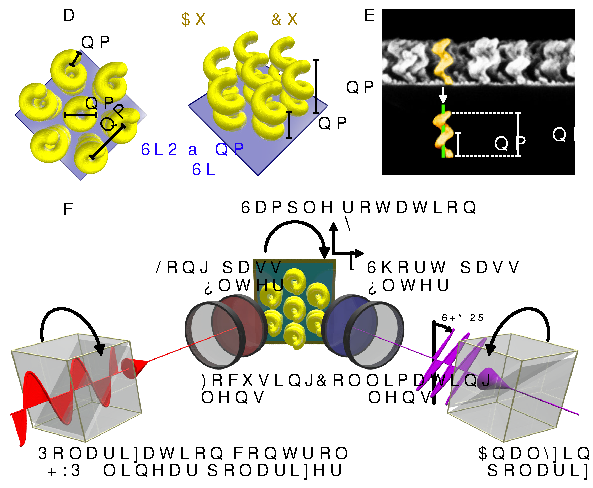
\includegraphics[scale=1.0]{./figures/results/OAinPlanarNanohelices/setup.pdf}
    \caption{\label{fig:results:OAinPlanarNanohelices:setup}
    \textbf{a)} Schematic diagram of one handedness of nanohelix array, showing structure spacing $\SI{55}{\nano\m}$, height $\SI{81}{\nano\m}$, and pitch $\SI{37}{\nano\m}$. \textbf{b)} Side-on SEM of the metamaterial surface, of the same handedness. A single helix has been highlighted for clarity. \textbf{c)} Schematic of experimental setup, showing S-polarized $\SI{800}{\nano\m}$ incident light. For optical rotation measurements, the analyzing polarizer is continuously rotated, for a series of sample azimuthal rotations.}	
\end{figure}

Figure~\ref{fig:results:OAinPlanarNanohelices:combined_data}a shows SHG hotspots corresponding to the polarization of SHG emission as the sample is rotated. The green markers on Figure~\ref{fig:results:OAinPlanarNanohelices:combined_data}a show the angle of SHG polarization for each sample rotation angle. Relative to the incoming S-polarized light (perpendicular to the plane of incidence), an SHG-OR of approximately $+\SI{45}{\degree}$ is observed for the left-handed structures. \textit{This SHG-OR angle does not change significantly over the regions of SHG emission, i.e. over hundreds of degrees of sample rotation.} 
Moreover, upon measuring the right-handed structures, the SHG-OR reverses to approximately $-\SI{45}{\degree}$. This behavior is exactly as expected for SHG-OR due to intrinsic chirality. The intensity of SHG emission does vary upon rotation, suggesting a dipole coupling between the incident light and the end terminations of the nanohelices. 

\begin{figure}[htb!]	
    \centering	
    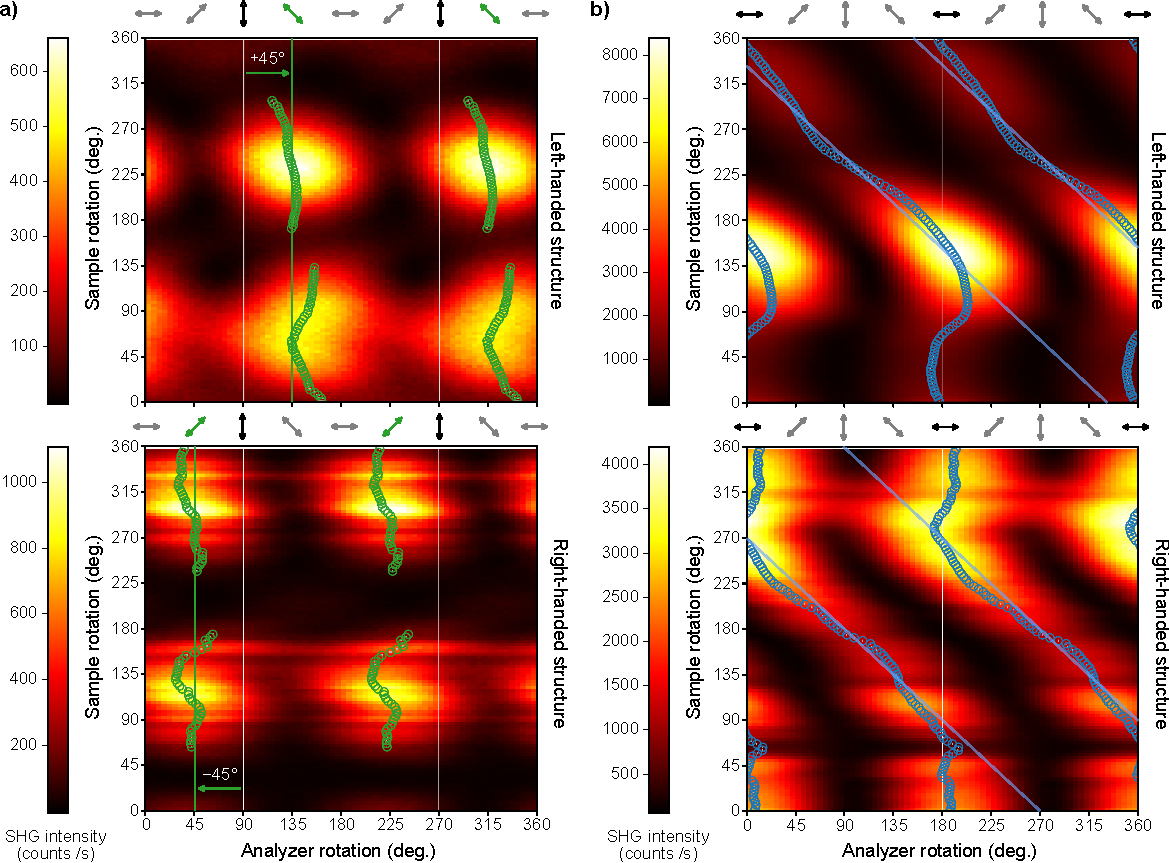
\includegraphics[scale=0.8]{./figures/results/OAinPlanarNanohelices/combined_data.pdf}

    \caption{\label{fig:results:OAinPlanarNanohelices:combined_data}
    \textbf{a)} SHG optical rotation heatmaps for both enantiomorphs of helical metamaterial. S-polarized incident light results in rotated linearly polarized SHG emission. By continuously rotating the analyzer, the angle of maximum intensity at each sample rotation can be obtained (shown in green markers). For the left-handed structure an SHG-OR angle of around $+\SI{45}{\degree}$ is found. In the mirrored, right-handed structure, the SHG-OR changes sign, to around $-\SI{45}{\degree}$. Importantly, in both cases the angle remains relatively unchanged upon sample rotation, though the overall intensity varies periodically. \textbf{b)} SHG optical rotation heatmap for both enantiomorphs of the helical metamaterial, for P-polarized incident light. In this case, both the angle of SHG-OR and the intensity of SHG emission are strongly dependent on sample rotation. Additionally, there is no clear reversal between enantiomorphs of the metamaterial. Instead, the sign of SHG-OR reverses under sample rotation, suggesting contributions from anisotropy dominating over contributions from the structure’s intrinsic chirality.}	
\end{figure}

Importantly, SHG-OR is not always independent of sample anisotropy. As discussed in section~\ref{sec:results:OAinPlanarNanohelices:discussion}, SHG is a highly symmetry-sensitive technique, whereby symmetry is expressed in the values of nonlinear susceptibility tensor elements. Depending on the experimental geometry, and on the values of these tensor elements, competing symmetries within the structure can be dominant in the measured results. Indeed, we demonstrate this in Figure~\ref{fig:results:OAinPlanarNanohelices:combined_data}b. The data presented in Figure~\ref{fig:results:OAinPlanarNanohelices:combined_data}b were obtained from the same nanohelices, however whereas in Figure~\ref{fig:results:OAinPlanarNanohelices:combined_data}a we used S-polarized light, here P-polarized light was employed. As in Figure~\ref{fig:results:OAinPlanarNanohelices:combined_data}a, the heat maps correspond to SHG intensity as a function of sample and analyzer rotation angles. Contrary to Figure~\ref{fig:results:OAinPlanarNanohelices:combined_data}a, the SHG-OR angle changes significantly over the regions of SHG emission, closely following the sample rotation angle. This behavior is exactly as expected for SHG-OR, dominantly due to sample anisotropy. The experimental geometry must be carefully selected to address the structural chirality exclusively.

The nonlinear chiroptical behavior reported here is in stark contrast to the linear chiroptical case. The linear OR of the nanohelices was investigated with optical microscopy and spectroscopy. White light from a halogen lamp is linearly polarized and directed to the sample through an Axio Imager M2 microscope. 
An analyzing polarizer is placed in the reflected light path. The latter can be precisely rotated through $\SI{360}{\degree}$. Under crossed polarizer geometry, only light that has experienced OR reaches the detector. By rotating the analyzer, the sign of this OR can be obtained. 
Figure~\ref{fig:results:OAinPlanarNanohelices:lin_data}a shows a $3 \times 3$ array of optical microscopy images (in color) of the nanohelices. The rows correspond to three different sample rotation angles ($\SI{0}{\degree}$, $\SI{45}{\degree}$ and $\SI{90}{\degree}$) and the columns corresponds to three analyzer rotation angles ($\SI{85}{\degree}$, $\SI{90}{\degree}$, $\SI{95}{\degree}$).
The sign of OR is revealed by the color contrast in the images. For a sample oriented at $\SI{0}{\degree}$ and an analyzer positioned at $\SI{85}{\degree}$, the image appears green.
Upon rotating the analyzer to $\SI{95}{\degree}$, the color changes to red. However, upon orienting the sample at $\SI{90}{\degree}$, the color contrast reverses, indicating an opposite OR. This behavior suggests that the angle of OR depends on sample orientation and that OR changes sign every $\SI{90}{\degree}$. 
The trend is confirmed by Figure~\ref{fig:results:OAinPlanarNanohelices:lin_data}b, which shows an OR spectral map, obtained upon rotating the sample between crossed polarizers. 
Here, a $\SI{90}{\degree}$ rotational periodicity for the OR is clearly visible, at wavelengths above $\SI{550}{\nano\m}$. The behavior of the sample is consistent with that of a radiating dipole rotated through $\SI{360}{\degree}$. Such a dipole can be situated at the end-termination of the nanohelices. In the ranges of study, this dipole is excited by wavelengths from $\SI{550}{\nano\m}$ to $\SI{800}{\nano\m}$. The latter is the fundamental wavelength used for the SHG data in Figure~\ref{fig:results:OAinPlanarNanohelices:combined_data}, where the SHG intensity also depends on coupling to the end-termination dipole, as discussed above.

\begin{figure}[htb!]	
    \centering	
    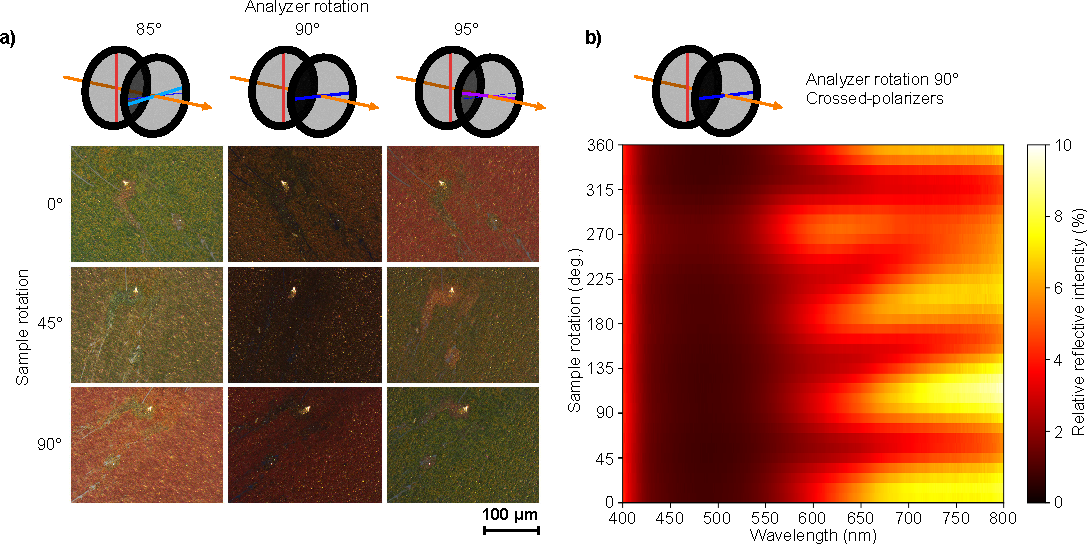
\includegraphics[scale=0.8]{./figures/results/OAinPlanarNanohelices/lin_data.pdf}

    \caption{\label{fig:results:OAinPlanarNanohelices:lin_data}
    Linear optical rotation data obtained through microscopy. \textbf{a)} Microscopy images of left-handed structure under illumination by linearly polarized white light, with various almost-crossed analyzing polarizer angles. By rotating the analyzer slightly away from crossed ($\SI{90}{\degree}$), the spectral dependence of optical rotation can be observed. Longer wavelengths are transmitted more through the analyzer when oriented at $+\SI{5}{\degree}$ away from crossed. Crucially, upon rotating the structure by $\SI{90}{\degree}$, the OR appears to reverse: longer wavelengths are now transmitted more through the analyzer when oriented at $-\SI{5}{\degree}$ from crossed. \textbf{b)} Linear OR map obtained from a spectrometer connected to the microscope viewport, showing clear dependence on sample rotation. Since the sample is between crossed polarizers, positive and negative OR both increase the measured intensity.}
\end{figure}

\subsection{Discussion}\label{sec:results:OAinPlanarNanohelices:discussion}
\textbf{Lots of this can also be moved into the main background section.}

At a given optical frequency $\omega$, the nonlinear chiroptical effects are commonly described in terms of the nonlinear susceptibility tensors, relating the induced polarization ($P$) at the second-harmonic ($2\omega$) to the driving electric ($E$) and magnetic ($B$) fields, by equation~\ref{eq:results:OAinPlanarNanohelices:P2contributions}.\cite{Boyd2008a}
\begin{equation}\label{eq:results:OAinPlanarNanohelices:P2contributions}	
    {P_i}\left( {2\omega } \right) = 
    \varepsilon{_0}\chi_{ijk}^{eee}{E_j}\left(\omega \right){E_k}\left(\omega \right) + \varepsilon{_0}\chi_{ijk}^{eem}{E_j}\left(\omega \right){B_k}\left(\omega \right) + \varepsilon{_0}\chi_{ijk}^{eme}{B_j}\left(\omega \right){E_k}\left(\omega \right)
\end{equation}
The indices $i$, $j$, and $k$ describe the Cartesian coordinates of the fields, and can represent $x$, $y$, or $z$ (see Figure~\ref{fig:results:OAinPlanarNanohelices:setup}c). 
The superscripts $e$ and $m$ stand for electric and magnetic dipole transitions, respectively, while $\varepsilon{_0}$ is the permittivity of vacuum. 
In addition to equation~\ref{eq:results:OAinPlanarNanohelices:P2contributions}, the incident electromagnetic fields can induce a magnetization $M_i$ analogous to the polarization $P_i$. 
In our experiment (Figure~\ref{fig:results:OAinPlanarNanohelices:combined_data}a), the incident electric field is polarized perpendicularly to the main helix axis, therefore we can exclude this magnetic contribution. Away from resonance, the magnetic component of the incident light is much weaker than the electric component. 
In our analysis, we therefore consider only the contribution from electric dipoles ($eee$). Furthermore, for collinear SHG experiments, the incident fields ${E_j}(\omega)$ and ${E_k}(\omega)$ are indistinguishable. This allows equation~\ref{eq:results:OAinPlanarNanohelices:P2contributions} to be reduced under permutation symmetry to equation~\ref{eq:results:OAinPlanarNanohelices:PshgFull}, as in section~\ref{sec:background:NonlinearOptics:tensorsymmetry:permutation}.

\begin{equation}\label{eq:results:OAinPlanarNanohelices:PshgFull}
	\begin{pmatrix}
		P_{x}\\ 
		P_{y}\\ 
		P_{z}
	\end{pmatrix} =
	\begin{pmatrix}
		\chi_{xxx} & \chi_{xyy} & \chi_{xzz} & \chi_{xyz} & \chi_{xzx} & \chi_{xyx}\\ 
		\chi_{yxx} & \chi_{yyy} & \chi_{yzz} & \chi_{yzy} & \chi_{yzx} & \chi_{yxy}\\ 
		\chi_{zxx} & \chi_{zyy} & \chi_{zzz} & \chi_{zyz} & \chi_{zxz} & \chi_{zyx}
	\end{pmatrix}
	\begin{pmatrix}
		E_{x}E_{x}\\ 
		E_{y}E_{y}\\ 
		E_{z}E_{z}\\
		2E_{y}E_{z}\\ 
		2E_{z}E_{x}\\ 
		2E_{x}E_{y}
	\end{pmatrix}
\end{equation}
The presence of sample symmetry can further reduce the number of non-zero tensor components. The presence of surface isotropy (full rotational symmetry about the surface normal) causes 11 components to be eliminated (section~\ref{sec:background:NonlinearOptics:tensorsymmetry:isotropy}) we can refer to these as the ``anisotropy components''. Likewise, for a tensor with mirror symmetry, 8 components are eliminated  (section~\ref{sec:background:NonlinearOptics:tensorsymmetry:chirality}). These ``chirality components'' are therefore only present in chiral structures. Importantly, both anisotropy and chirality tensor components can contribute to SHG-OR. 

Our sample is a chiral, anisotropic surface. With S-polarized light, ${E_j}(\omega)$ and ${E_k}(\omega)$ are polarized along the sample $y$-axis. Therefore, only the $\chi_{xyy}$, $\chi_{yyy}$ and $\chi_{zyy}$ tensor components are addressed. Here, we examine each component individually. 
First, we can see that $\chi_{zyy}$ is neither an in-plane anisotropy, nor a chirality parameter. Second, $\chi_{yyy}$ is an anisotropy but not a chirality parameter. And third, $\chi_{xyy}$ relates to \textit{both} anisotropy and chirality. 
Rotating the sample by an angle $\theta$ around the surface normal is equivalent to applying a rotation operation to the tensor in equation~\ref{eq:results:OAinPlanarNanohelices:PshgFull}. The treatment can be simplified by introducing effective nonlinear susceptibility tensor components as given in equation~\ref{eq:results:OAinPlanarNanohelices:ChiEff}.

\begin{equation}\label{eq:results:OAinPlanarNanohelices:ChiEff}
	\begin{split}
		&\chi_{xyy}^{eff}(\theta) = \cos\theta\sin^2\theta(\chi_{xxx} - 2\chi_{yyx}) \\
		&+ {\cos^2}\theta\sin\theta (2\chi _{xyx} - \chi_{yyy}) + {\cos^3}\theta(\chi_{xyy}) - {\sin^3}\theta(\chi _{yxx}), \\
		\\
		&\chi_{yyy}^{eff}(\theta) = \cos\theta\sin^2\theta(2\chi_{xyx} - \chi_{yxx}) \\
		&+ {\cos^2}\theta\sin\theta (2\chi _{yyx} - \chi_{xyy}) + {\cos^3}\theta(\chi_{yyy}) - {\sin^3}\theta(\chi _{xxx}), \\
		\\
		&\chi _{zyy}^{eff}(\theta) = \cos\theta\sin\theta (2\chi_{zxy}) + {\sin^2}\theta(\chi_{zxx}) + {\cos^2}\theta (\chi_{zyy}).
	\end{split}
\end{equation}

Within the dipole approximation, the angle of SHG-OR is $\phi=\arctan{\left(\frac{E_P\left(2\omega\right)}{E_S\left(2\omega\right)}\right)}$. 
The values of the electric fields at the second harmonic are obtained from equation~\ref{eq:results:OAinPlanarNanohelices:PshgFull} following $\mathbf{E}(2\omega)\sim[\mathbf{n}\times\mathbf{P}(2\omega)]\times\mathbf{n}$, where $\mathbf{P}(2\omega)$ is a vector describing the induced polarization from equation~\ref{eq:results:OAinPlanarNanohelices:PshgFull}, and $\mathbf{n}$ is a unit vector describing the angle of observation. 
In our experimental configuration, the angle of optical incidence is $\SI{45}{\degree}$, hence $E_P(2\omega)\propto\frac{1}{2}(\chi_{zyy}^{eff}(\theta)-\chi_{xyy}^{eff}(\theta))$ and $E_P(2\omega)\propto\chi_{yyy}^{eff}(\theta)$. 
The angle of SHG-OR in this configuration is therefore given by equation~\ref{eq:results:OAinPlanarNanohelices:SHGangle}.
\begin{equation}\label{eq:results:OAinPlanarNanohelices:SHGangle}
	\phi  = \arctan \left({\frac{\chi_{zyy}^{eff}(\theta) - \chi _{xyy}^{eff}(\theta)}{2\chi _{yyy}^{eff}(\theta)}}\right)
\end{equation}
Likewise, the intensity of SHG emission is given by equation~\ref{eq:results:OAinPlanarNanohelices:SHGintensity}.
\begin{equation}\label{eq:results:OAinPlanarNanohelices:SHGintensity}
	I_{SHG} \propto \frac{1}{4}{\left| {\chi _{zyy}^{eff}\left( \theta  \right) - \chi _{xyy}^{eff}\left( \theta  \right)} \right|^2} + {\left| {\chi _{yyy}^{eff}\left( \theta  \right)} \right|^2}
\end{equation}
Although not trivial, the effects of anisotropy and chirality can be disentangled. To achieve this, equation~\ref{eq:results:OAinPlanarNanohelices:ExampleComponents} presents a suitable set of intrinsic tensor component relationships, as an example.
\begin{equation}\label{eq:results:OAinPlanarNanohelices:ExampleComponents}
	\begin{split}
		& \chi_{xxx} = \pm 0.5; \chi_{xyy} = \mp0.58; \chi_{yyx} = \pm 0.55 \\
		& \chi _{yxx} = 1.0; \chi _{yyy} = 0.34; \chi _{zyy} = 0.05; \chi _{zxx} = 0.02; \chi_{zyy} = 0.05; \chi _{zyx} = 0.01
	\end{split}
\end{equation}
The top three tensor components are associated with chirality and they change sign depending on the handedness of the structure ($+$ and $-$ for left- and right-handed structures, respectively). 
The lower 6 tensor components contain information on the anisotropy and do not change sign. 
With the values in equation~\ref{eq:results:OAinPlanarNanohelices:ExampleComponents}, we can calculate the SHG intensity and SHG-OR, for both enantiomorphs, see Figure~\ref{fig:results:OAinPlanarNanohelices:sim_data}. 
The figure has the same layout as Figure~\ref{fig:results:OAinPlanarNanohelices:combined_data}a and it can be seen that it matches very well the experimental behavior. 
\begin{figure}[htb!]	
    \centering	
    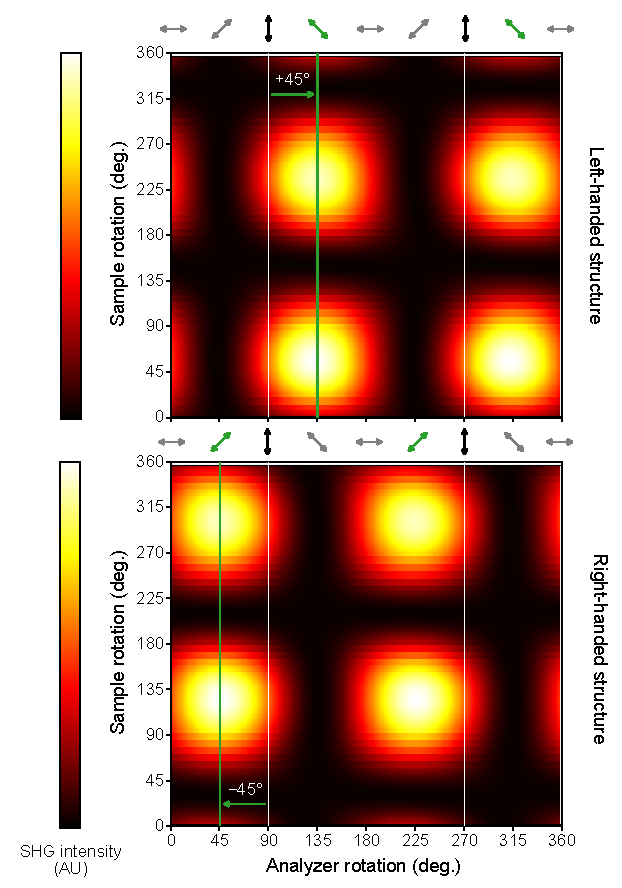
\includegraphics[scale=0.8]{./figures/results/OAinPlanarNanohelices/sim_data.pdf}

    \caption{\label{fig:results:OAinPlanarNanohelices:sim_data}
    SHG optical rotation heatmaps for the susceptibility tensor relationships given in equation~\ref{eq:results:OAinPlanarNanohelices:ExampleComponents}. The SHG-OR behavior closely matches that observed in Figure~\ref{fig:results:OAinPlanarNanohelices:combined_data}a.}
\end{figure}

In an \textit{isotropic} metasurface, composed of nanohelices, two principal models can be used to theoretically quantify the nonlinear optical activity. The first model builds upon Kauzmann's ``one-electron chirality''.\cite{Kauzmann1957a}
In its nonlinear treatment, the nonlinear optical activity requires magnetic dipoles caused by the electron's helical motion.\cite{Hache2001a}
The second model, builds upon Kuhn's~\cite{Kuhn1930} chirally-coupled electric dipole moments. In its nonlinear treatment, the nonlinear optical activity requires only electric dipole moments.\cite{Hache2001a}
In plasmonic nanomaterials this could be the coupling between any chirally-arranged metallic features. Importantly, the ``one-electron''”'' model permits only SHG-CD, whereas the coupled-dipole model allows SHG-CD, SHG linear dichroism (SHG-LD), and SHG-OR.\cite{Fischer2005a}
Unlike linear chiroptical measurements, information is gained by measuring both SHG-CD and SHG-OR: the mechanism of a structure's chiroptical response can be determined by comparing these two nonlinear chiroptical effects. 

However, when treating \textit{anisotropic} surfaces, the analysis is much more complex than in the isotropic case. SHG-OR is possible in both models, and there is no simple distinction between the two. Slight changes in the structure design can result in significant changes in the optical behavior, due to the large number of interacting tensor components responsible for the SHG-OR. As we have observed, this complexity can result in interesting and highly desirable optical properties, under the right experimental and geometric conditions. The flexibility of geometry makes metamaterials an ideal platform for exploring this interplay between structural and experimental geometry. 

Finally, it is important to consider that the SHG-OR in Figure~\ref{fig:results:OAinPlanarNanohelices:combined_data}a could, in principle, originate from the out of plane anisotropy axis. SHG-OR effects from this axis would not change under azimuthal sample rotation. However, such an anisotropy-induced SHG-OR would not change sign, depending on the handedness of the nanohelices. Consequently, because our SHG-OR changes sign depending on handedness, we can conclusively attribute it to chirality. 

\subsection{Conclusions}\label{sec:results:OAinPlanarNanohelices:conclusions}
To conclude, we report an unambiguous SHG-OR effect of $\pm \SI{45}{\deg}$, from planar chiral metamaterials. The effect is due to the intrinsic chirality of the helical nanostructures; the angle of SHG-OR is rotationally invariant, and, as expected, it reverses for the mirrored structures. Contrary to their linear chiroptical counterparts, SHG-CD and SHG-OR are not trivially related to one another. Therefore, our results on SHG-OR pertain to an important and previously unobserved chiroptical effect in this kind of systems. We have demonstrated that, under the right experimental conditions, it is possible to extract purely chiral information from highly anisotropic structures. Further work on disentangling chiral and anisotropic contributions to nonlinear chiroptical effects will unveil the physical mechanisms at work and will lead to their optimization. 

\subsection{Methods}\label{sec:results:OAinPlanarNanohelices:methods}
\textcolor{red}{
\textbf{This section in the paper has details about the experiment. This could be rewritten to reference the generic method thesis section, and acts as specific details. Possibly move these bits inline with the text too?}
}

\subsubsection{SHG-OR measurements}
Linearly polarized $\SI{100}{\femto\s}$ pulsed light centered at $\SI{800}{\nano\m}$ was directed to a half-wave plate and rotated to a specific linear polarization angle. A RG665 long pass filter removed any existing SHG from the beam, before an achromatic lens focused the $\SI{800}{\nano\m}$ light onto our sample at 45° incidence. A BG39 filter then removed reflected $\SI{800}{\nano\m}$ light, passing only the $\SI{400}{\nano\m}$ SHG emission which was then collimated by another lens. The SHG emission then passed through an analyzing polarizer, before being focused onto a photomultiplier tube (PMT). The PMT output is pre-amplified and sent to an SRS SR400 Gated Photon Counter. For our SHG optical rotation measurements, both the sample azimuthal angle and the analyzing polarizer angle were continuously rotated. 

\subsubsection{Linear microscopy}
Microscopy images were obtained on a commercial Zeiss Axio Imager M2m wide-field microscope, with a halogen lamp for illumination. Images were taken in bright-field reflection mode, through an Epiplan-Neofluar 20x/0.50 HD DIC objective, using an Axiocam 105 color camera. Incident polarization was controlled using a fixed Zeiss linear polarizer slider, with the output image analyzed with a Zeiss $\SI{360}{\deg}$ rotatable analyzer slider. Linear spectra were obtained by diverting the microscope image to a collection lens focusing onto a $\SI{400}{\micro\m}$ diameter multimode optical fiber. The output of the fiber was connected to an Ocean Optics QE Pro commercial spectrometer, running with a $\SI{500}{\milli\s}$ integration time. The spectral data is normalized to account for the spectral lineshape of our halogen lamp source. Reference spectra were obtained using a silver mirror to measure the spectral lineshape of the source only. The measured metamaterial spectra were divided by this reference to give spectra independent of the illumination source.

\subsubsection{Nanostructure fabrication}
An array of nanohelices is fabricated using nanoglancing angle deposition (nanoGLAD), which is a wafer-scale bottom-up growth scheme that combines block copolymer micelle nanolithography (BCML)~\cite{Glass2003} with glancing angle deposition (GLAD).\cite{Mark2013} 
The former, BCML, was used to pattern a quasi-hexagonal array of Au nanoseeds with desired diameter and spacing on a 2 inch silicon wafer, which serve as seeds for the GLAD process. Cu and Au are co-deposited onto the BCML seeds at a vapor flux angle of $\SI{87}{\deg}$ with continuous azimuthal rotation of the substrate. The ratio of Cu to Au was determined during deposition using two independent quartz crystal microbalances and the respective evaporators were controlled to maintain the desired mixing ratio during the entire deposition processes.